\section{Systematics}

\begin{frame}{Systematics}

    \begin{itemize}
        \smaller
        \item Statisitical uncertainties are calculated using different approaches for the two
            analyses
        \item Shape analysis:
        \begin{itemize}
            \smaller
            \item uncertainty is included in fit with nuisance parameters (n.p.)
            \item most uncertainties are accounted for using morphing templates
            \item MC statistical uncertainty accounted for on a bin-by-bin basis using Barlow-Beeston
                approach
            \item correlations between channels is accounted for at time of minimization
        \end{itemize}
        \item Counting analysis:
        \begin{itemize}
            \smaller
            \item uncertainty accounted for by carrying out measurement with each uncertainty source
                varied by $\pm 1\sigma$
            \item different jet and trigger categories are combined considering correlations.
        \end{itemize}
    \end{itemize}

\end{frame}


\begin{frame}{Systematics}

    \begin{itemize}
        \smaller
        \item lumi and cross-sections of \ttbar, \tW, \zjets,\wjets, \gjets. dibson
        \item gen-level reweightings: PU, top \pt, \WW \pt  
        \item HLT efficiencies: single muon trigger and single electron trigger.
        \item object systematics
        \begin{itemize}
        \smaller
            \item muon: identification, isolation, energy scale
            \item electron: identification, reconstruction, energy scale
            \item tau: identification, misidentification, energy scale.
            \item jet: energy scale, energy resolution
            \item btag: tag/mistag.
        \end{itemize}
        \item tau decay branching fractions: \bte, \btm,  \bth of major \PGth modes
        \item simulation: ISR/FSR, ME-PS matching, UE tuning.
        
        
    \end{itemize}

\end{frame}


\begin{frame}{Systematics}

    \begin{itemize}
    \smaller
        \item brought up in a CMS week talk.
        \item tau reconstruction efficiencies are different for different \PGth decay mode.
        \item major \PGth decay branching fractions 
            \begin{equation*}\tiny
            \begin{split}
            &   \mathcal{B}(\PGth\to \PGp^\pm)        = 0.1082(5), \quad 
                \mathcal{B}(\PGth\to \PGp^\pm \PGp^0)  = 0.2549(9), \quad 
                \mathcal{B}(\PGth\to \PGp^\pm2\PGp^0)  = 0.0926(10),\\
            &   \mathcal{B}(\PGth\to3\PGp^\pm)        = 0.0931(5), \quad
                \mathcal{B}(\PGth\to3\PGp^\pm \PGp^0)  = 0.0462(5).           
            \end{split}
            \end{equation*}
        \item find the decay mode of \PGth in simulation based on gen-level information. 
        \item propagate uncertainty of each $\mathcal{B}(\PGth)$
        \item impact less than 0.1\%. neglectable.
    \end{itemize}
        

    \begin{figure}
    \centering
    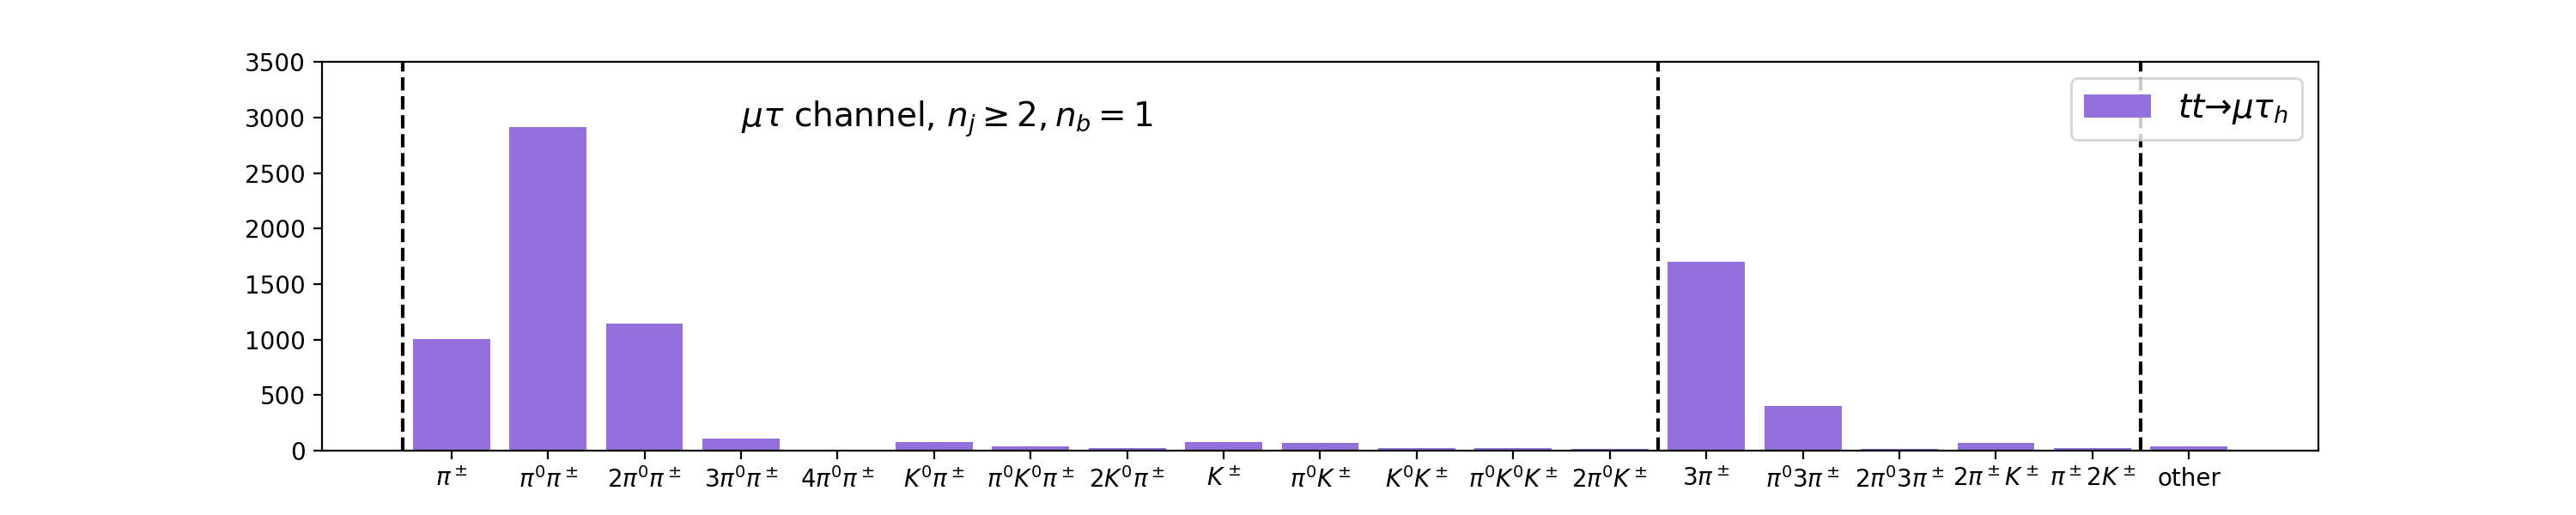
\includegraphics[width=0.99\textwidth]{chapters/Analysis/sectionSystematics/figures/tauBr/tauhDecay_mutau.png}
    \end{figure}
\end{frame}


\begin{frame}{Systematics}

    \begin{itemize}
    \smaller
        \item tau reconstruction is sensitive to $\alpS$ in the FSR systematics. 
        \item remove the effect of \PGth identification when evaluating FSR systematics.
        \item avoid double counting \PGth identification systematics.
        \item measure the \PGth identification efficiency in nominal and FSR+- simulation.
        \item reweight the FSR+- simulation with scale factors.
    \end{itemize}
        

    \begin{figure}
    \centering
    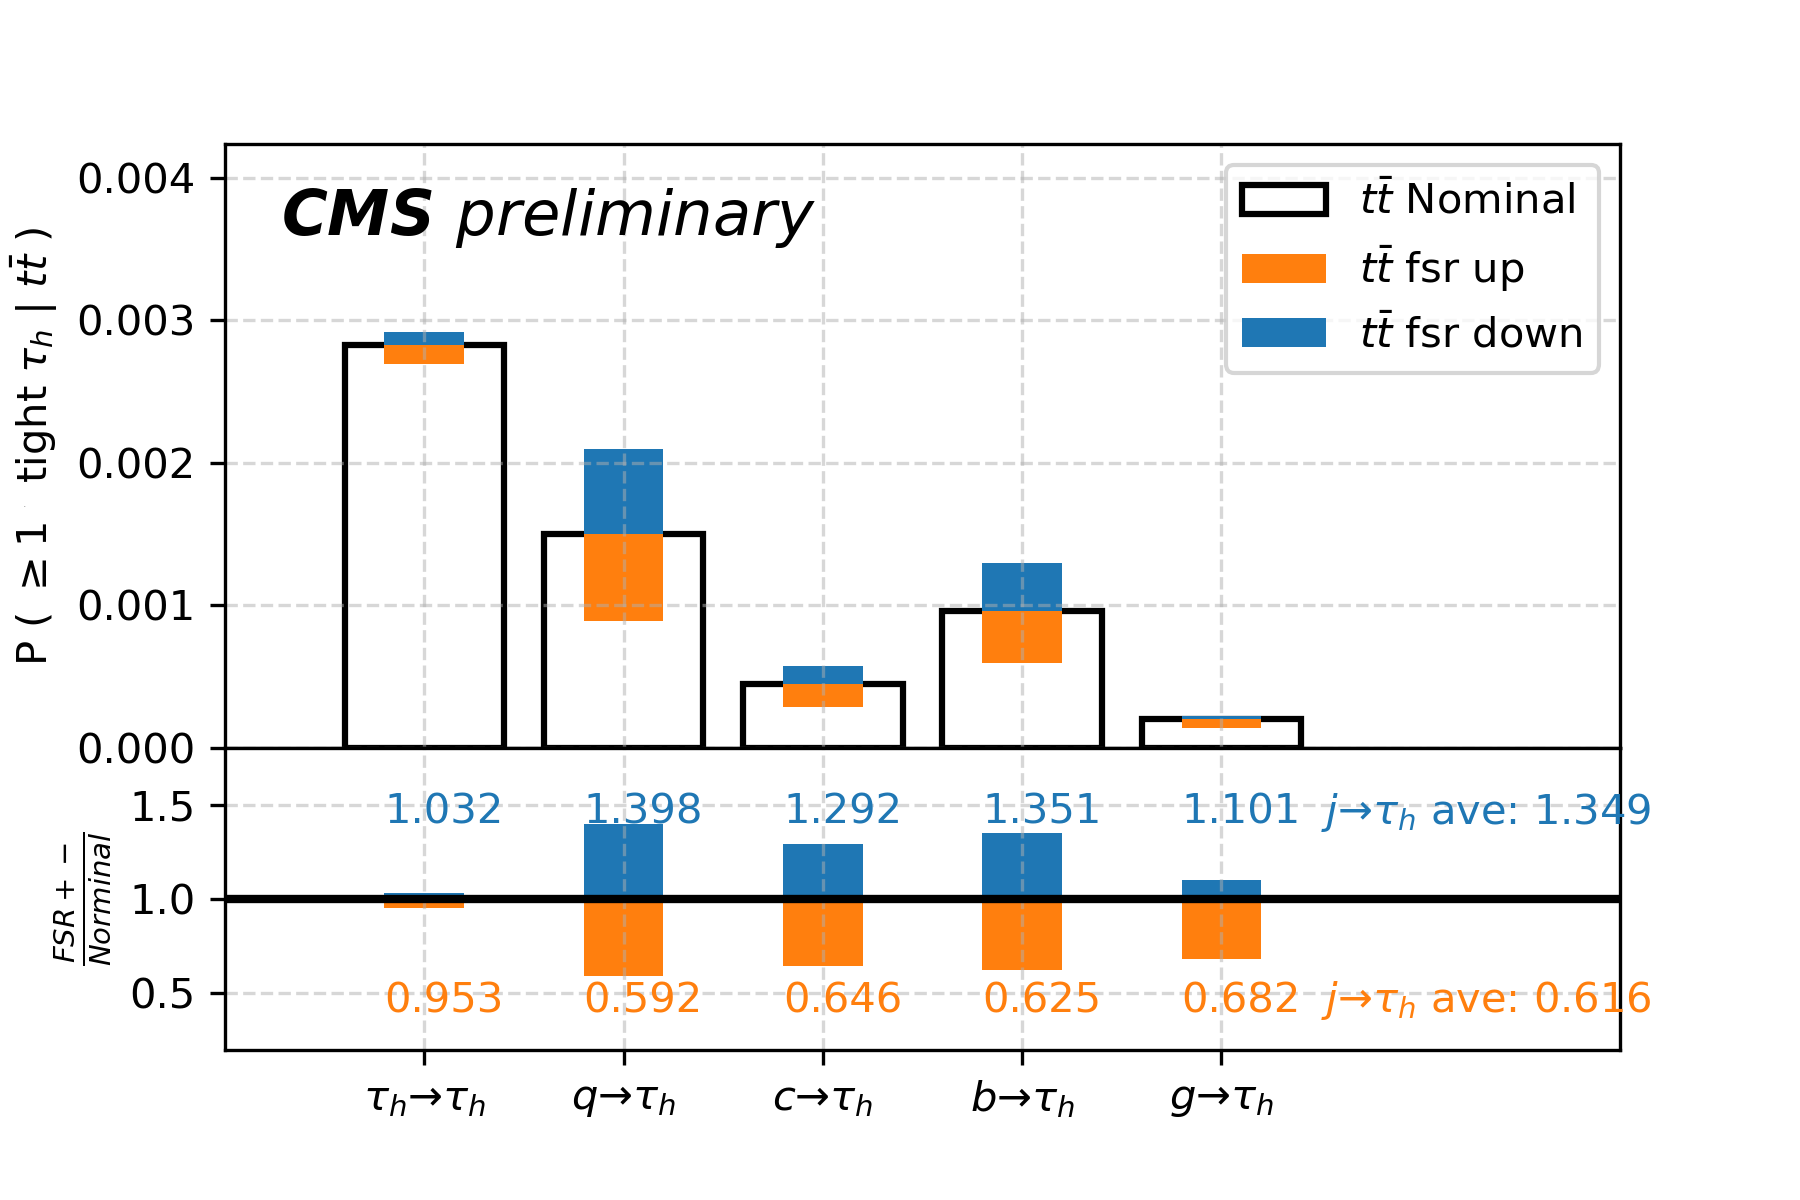
\includegraphics[width=0.49\textwidth]{chapters/Analysis/sectionSystematics/figures/ttTheoretical/2020_MCRatio_fsr_tauGenFlavor_tauTight.png}
    % 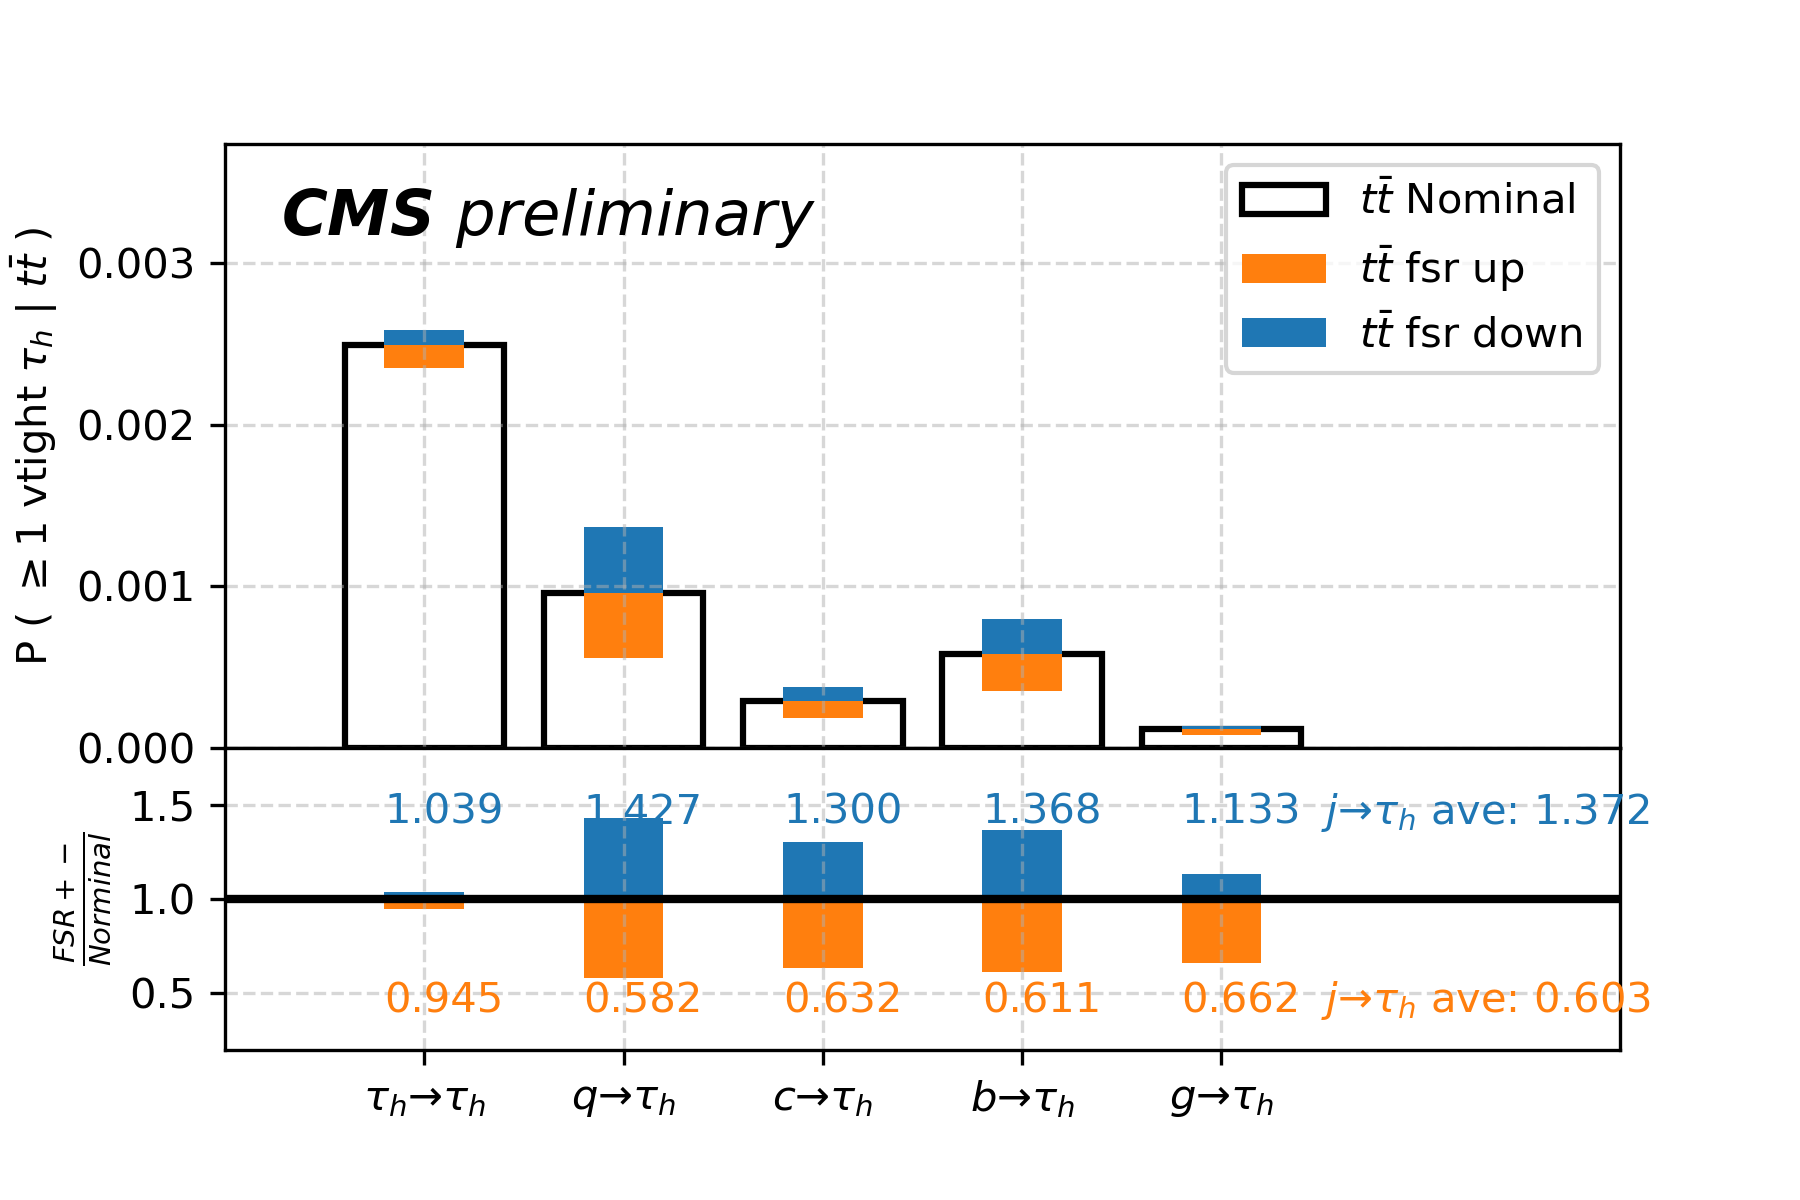
\includegraphics[width=0.49\textwidth]{chapters/Analysis/sectionSystematics/figures/ttTheoretical/2020_MCRatio_fsr_tauGenFlavor_tauVTight.png}
    \end{figure}
\end{frame}

\begin{frame}{Systematics}
    \centering
    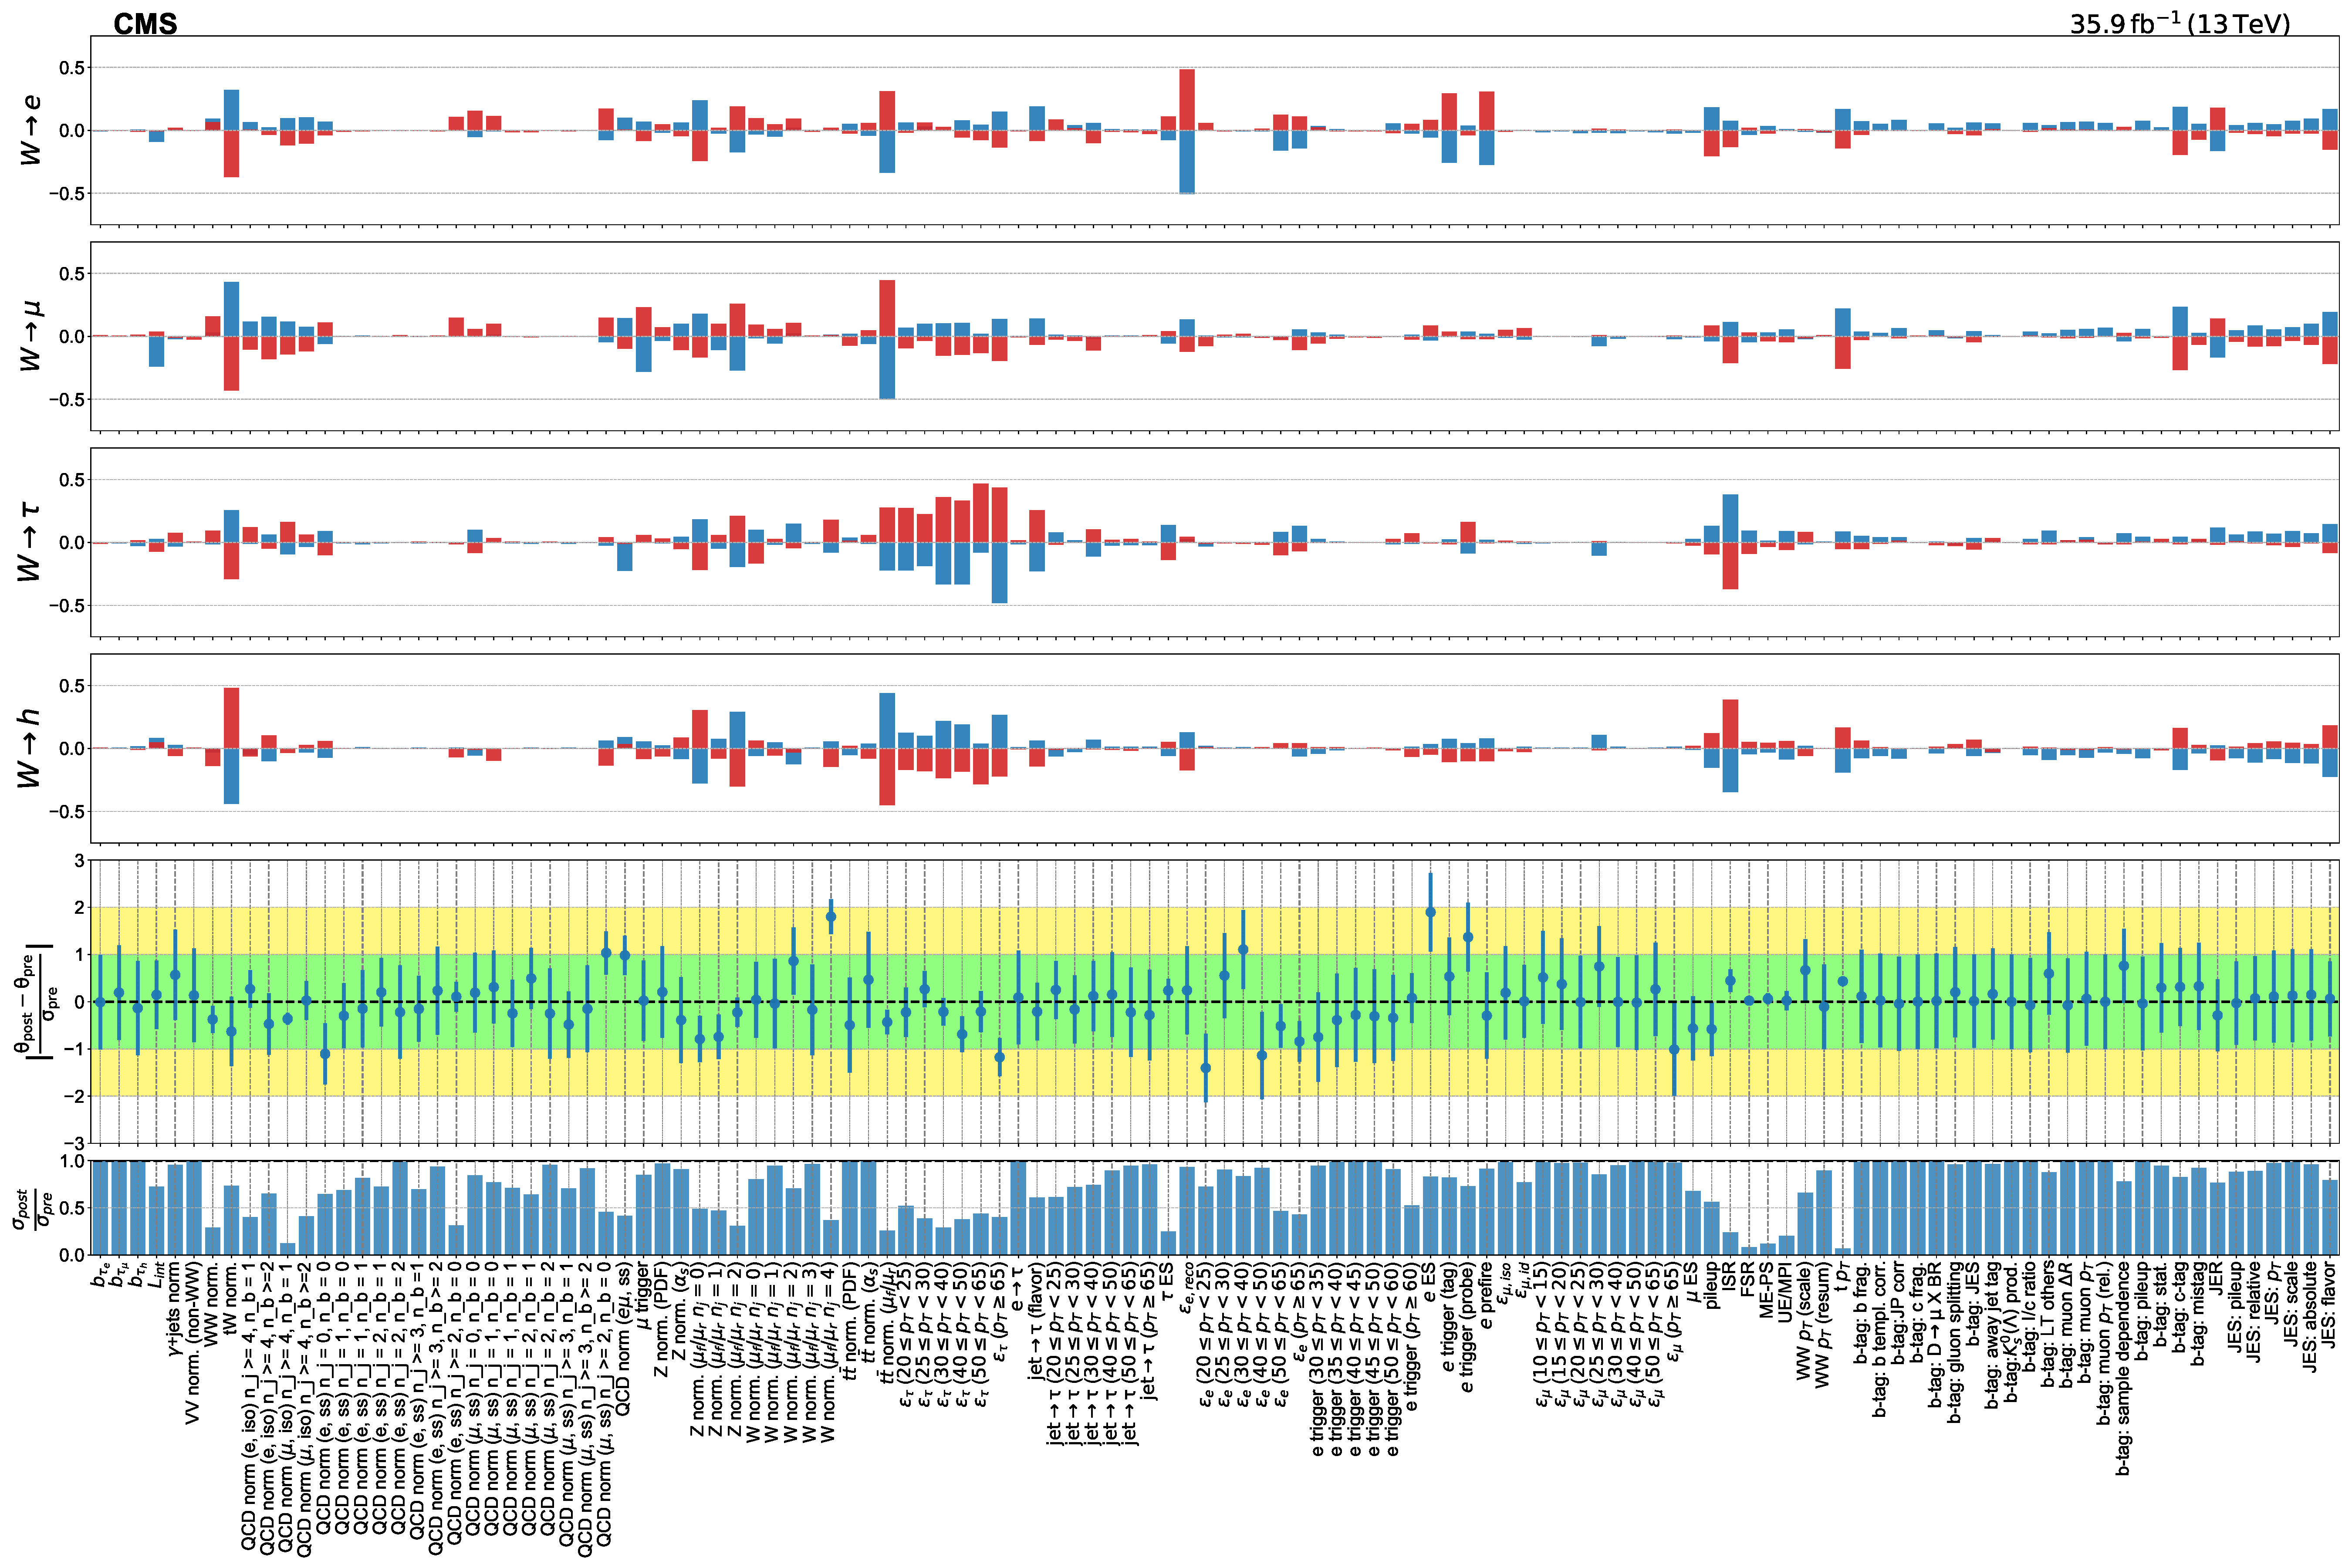
\includegraphics[width=\textwidth]{chapters/Analysis/sectionSystematics/figures/pulls_impacts_final.pdf}
\end{frame}

\begin{frame}{Systematics}
    \centering
    \includegraphics[width=0.7\textwidth]{chapters/Analysis/sectionSystematics/figures/correlation_matrix_full.pdf}
\end{frame}

\begin{frame}{}
    \centering
    \begin{table}[]
        \renewcommand{\arraystretch}{1.1}
        \setlength{\tabcolsep}{0.4em}
        \centering
        \resizebox{0.6\textwidth}{!}{\begin{table}[]

    
  \renewcommand{\arraystretch}{1.1}
  \setlength{\tabcolsep}{0.4em}
  \centering
  \caption{ Statistical and systematic error of four categories. }
  \resizebox{\textwidth}{!}{
      \begin{tabular}{|l|ccc|ccc|ccc|ccc|ccc|}
      \hline
      Error Source & \multicolumn{3}{c|}{$\mu$-1b} & \multicolumn{3}{c|}{$\mu$-2b} & \multicolumn{3}{c|}{$e$-1b} & \multicolumn{3}{c|}{$e$-2b} \\
      \hline
                    & $B_e$ & $B_\mu$ & $B_\tau$ & $B_e$ & $B_\mu$ & $B_\tau$ & $B_e$ & $B_\mu$ & $B_\tau$ & $B_e$ & $B_\mu$ & $B_\tau$ \\
      \hline
      StatErr of Data                            & 0.543 & 0.533 & 1.243 & 0.714 & 0.637 & 1.492 & 0.743 & 0.557 & 1.520 & 0.904 & 0.707 & 1.807 \\ 
      StatErr of bg MC                           & 0.178 & 0.745 & 0.767 & 0.110 & 0.411 & 0.501 & 0.897 & 0.257 & 1.065 & 0.494 & 0.137 & 0.521 \\ 
      StatErr of sg MC                           & 0.168 & 0.151 & 0.415 & 0.189 & 0.165 & 0.428 & 0.217 & 0.176 & 0.503 & 0.233 & 0.192 & 0.520 \\ 
      \hline
      PDG err of $Br^\tau_e$                     & 0.002 & 0.019 & 0.029 & 0.002 & 0.019 & 0.029 & 0.003 & 0.019 & 0.029 & 0.003 & 0.020 & 0.030 \\ 
      PDG err of $Br^\tau_\mu$                   & 0.047 & 0.017 & 0.098 & 0.047 & 0.017 & 0.099 & 0.041 & 0.013 & 0.101 & 0.043 & 0.013 & 0.106 \\ 
      2.5$\%$ err of luminosity                  & 0.330 & 0.461 & 0.120 & 0.093 & 0.064 & 0.049 & 0.135 & 0.390 & 0.204 & 0.002 & 0.101 & 0.092 \\ 
      5$\%$ err of tt XS                         & 0.002 & 0.000 & 0.151 & 0.009 & 0.015 & 0.032 & 0.021 & 0.011 & 0.148 & 0.011 & 0.002 & 0.003 \\ 
      5$\%$ err of tW XS                         & 0.002 & 0.001 & 0.157 & 0.010 & 0.015 & 0.033 & 0.022 & 0.012 & 0.155 & 0.011 & 0.002 & 0.004 \\ 
      5$\%$ err of t XS                          & 0.062 & 0.062 & 0.033 & 0.053 & 0.052 & 0.058 & 0.063 & 0.060 & 0.032 & 0.052 & 0.054 & 0.040 \\ 
      5$\%$ err of W+Jets XS                     & 0.343 & 0.354 & 0.325 & 0.068 & 0.068 & 0.066 & 0.349 & 0.347 & 0.366 & 0.065 & 0.066 & 0.084 \\ 
      10$\%$ err of Z+Jets XS                    & 0.495 & 2.655 & 0.237 & 0.122 & 0.491 & 0.055 & 1.576 & 0.501 & 0.173 & 0.275 & 0.104 & 0.041 \\ 
      10$\%$ err of $\gamma$+Jets XS             & 0.020 & 0.019 & 0.029 & 0.005 & 0.005 & 0.007 & 0.249 & 0.247 & 0.213 & 0.058 & 0.058 & 0.081 \\ 
      10$\%$ err of VV XS                        & 0.004 & 0.044 & 0.027 & 0.001 & 0.010 & 0.005 & 0.038 & 0.003 & 0.021 & 0.008 & 0.001 & 0.001 \\ 
      25$\%$ err of QCD in $e 4j$                & 0.000 & 0.000 & 0.000 & 0.000 & 0.000 & 0.000 & 1.164 & 1.118 & 2.410 & 0.219 & 0.218 & 0.406 \\ 
      25$\%$ err of QCD in $\mu 4j$              & 0.742 & 0.737 & 1.562 & 0.223 & 0.214 & 0.384 & 0.000 & 0.000 & 0.000 & 0.000 & 0.000 & 0.000 \\ 
      25$\%$ err of QCD in $e\tau$               & 0.000 & 0.000 & 0.000 & 0.000 & 0.000 & 0.000 & 0.372 & 0.498 & 2.651 & 0.069 & 0.092 & 0.503 \\ 
      25$\%$ err of QCD in $\mu\tau$             & 0.345 & 0.465 & 2.360 & 0.185 & 0.250 & 1.285 & 0.000 & 0.000 & 0.000 & 0.000 & 0.000 & 0.000 \\ 
      top pT reweighting                         & 0.000 & 0.000 & 0.032 & 0.002 & 0.003 & 0.007 & 0.004 & 0.002 & 0.031 & 0.002 & 0.000 & 0.001 \\ 
      0.6$\%$ err of $\epsilon_e$ reco           & 0.575 & 0.054 & 0.042 & 0.583 & 0.055 & 0.042 & 0.709 & 0.160 & 0.103 & 0.574 & 0.084 & 0.069 \\ 
      1.4$\%$ err of $\epsilon_e$ id             & 1.386 & 0.129 & 0.101 & 1.410 & 0.133 & 0.101 & 1.766 & 0.335 & 0.275 & 1.456 & 0.163 & 0.197 \\ 
      0.1$\%$ err of $\epsilon_\mu$ reco         & 0.015 & 0.125 & 0.016 & 0.008 & 0.095 & 0.011 & 0.009 & 0.078 & 0.008 & 0.008 & 0.077 & 0.008 \\ 
      0.2$\%$ err of $\epsilon_\mu$ id           & 0.052 & 0.496 & 0.066 & 0.021 & 0.370 & 0.045 & 0.033 & 0.299 & 0.029 & 0.032 & 0.299 & 0.031 \\ 
      5$\%$ err of $\epsilon_\tau$               & 0.745 & 1.004 & 5.091 & 0.694 & 0.937 & 4.823 & 0.723 & 0.967 & 5.146 & 0.700 & 0.937 & 5.111 \\ 
      4.7$\%$ err of $\epsilon_{j\to\tau}$       & 0.460 & 0.620 & 3.145 & 0.307 & 0.414 & 2.129 & 0.458 & 0.613 & 3.260 & 0.290 & 0.388 & 2.115 \\ 
      0.5$\%$ err of $ES_{e}$                    & 0.249 & 0.023 & 0.018 & 0.228 & 0.022 & 0.016 & 0.008 & 0.171 & 0.061 & 0.010 & 0.247 & 0.017 \\ 
      0.2$\%$ err of $ES_{\mu}$                  & 0.095 & 0.092 & 0.033 & 0.093 & 0.092 & 0.035 & 0.013 & 0.116 & 0.011 & 0.012 & 0.114 & 0.012 \\ 
      1.2$\%$ err of $ES_{\tau\to\pi^\pm}$       & 0.034 & 0.046 & 0.232 & 0.035 & 0.047 & 0.244 & 0.034 & 0.046 & 0.245 & 0.030 & 0.040 & 0.216 \\ 
      1.2$\%$ err of $ES_{\tau\to\pi^\pm\pi^0}$  & 0.086 & 0.116 & 0.587 & 0.069 & 0.093 & 0.477 & 0.066 & 0.088 & 0.469 & 0.075 & 0.100 & 0.548 \\ 
      1.2$\%$ err of $ES_{\tau\to3\pi^\pm}$      & 0.026 & 0.035 & 0.175 & 0.026 & 0.034 & 0.177 & 0.024 & 0.032 & 0.172 & 0.024 & 0.032 & 0.176 \\ 
      Single-e Trigger (probe syst)              & 0.218 & 0.020 & 0.016 & 0.222 & 0.021 & 0.016 & 0.029 & 0.032 & 0.004 & 0.036 & 0.004 & 0.009 \\ 
      Single-e Trigger (tag syst)                & 0.495 & 0.046 & 0.036 & 0.503 & 0.047 & 0.036 & 0.063 & 0.088 & 0.080 & 0.037 & 0.013 & 0.038 \\ 
      0.5$\%$ err of $Br_{\tau\to\pi^\pm}$       & 0.008 & 0.011 & 0.047 & 0.009 & 0.012 & 0.050 & 0.008 & 0.011 & 0.047 & 0.009 & 0.012 & 0.055 \\ 
      0.4$\%$ err of $Br_{\tau\to\pi^\pm\pi^0}$  & 0.018 & 0.024 & 0.102 & 0.019 & 0.025 & 0.108 & 0.019 & 0.025 & 0.110 & 0.020 & 0.025 & 0.117 \\ 
      1.1$\%$ err of $Br_{\tau\to\pi^\pm2\pi^0}$ & 0.022 & 0.029 & 0.124 & 0.022 & 0.029 & 0.120 & 0.022 & 0.028 & 0.123 & 0.024 & 0.031 & 0.143 \\ 
      0.5$\%$ err of $Br_{\tau\to3\pi^\pm}$      & 0.015 & 0.021 & 0.094 & 0.017 & 0.022 & 0.102 & 0.016 & 0.021 & 0.100 & 0.017 & 0.022 & 0.106 \\ 
      1.1$\%$ err of $Br_{\tau\to3\pi^\pm\pi^0}$ & 0.009 & 0.011 & 0.043 & 0.010 & 0.012 & 0.046 & 0.009 & 0.011 & 0.043 & 0.010 & 0.012 & 0.046 \\ 
      Pileup                                     & 0.041 & 0.183 & 0.777 & 0.231 & 0.026 & 0.891 & 0.428 & 0.474 & 0.592 & 0.248 & 0.137 & 0.835 \\ 
      JES                                        & 2.300 & 0.750 & 4.421 & 1.823 & 1.543 & 2.968 & 1.681 & 2.370 & 4.577 & 1.681 & 1.773 & 2.993 \\ 
      JER                                        & 0.238 & 0.180 & 0.265 & 0.143 & 0.146 & 0.356 & 0.259 & 0.249 & 0.406 & 0.148 & 0.138 & 0.538 \\ 
      Btag                                       & 0.098 & 0.772 & 0.643 & 0.111 & 0.023 & 0.114 & 0.181 & 0.091 & 0.762 & 0.024 & 0.109 & 0.088 \\ 
      Mistag                                     & 0.100 & 0.141 & 0.035 & 0.100 & 0.056 & 0.090 & 0.077 & 0.142 & 0.124 & 0.030 & 0.096 & 0.135 \\ 
      tt fsr                                     & 0.760 & 0.583 & 0.743 & 0.236 & 0.253 & 0.643 & 0.289 & 0.473 & 0.756 & 1.029 & 0.065 & 1.337 \\ 
      tt isr                                     & 0.724 & 0.747 & 1.105 & 0.720 & 0.723 & 0.876 & 0.317 & 1.060 & 1.414 & 0.043 & 0.830 & 0.062 \\ 
      tt UE                                      & 0.021 & 0.037 & 1.665 & 0.306 & 1.017 & 0.266 & 0.122 & 0.177 & 1.060 & 0.172 & 0.133 & 0.053 \\ 
      tt MEPS                                    & 0.198 & 0.653 & 1.699 & 1.117 & 0.645 & 0.129 & 0.033 & 0.743 & 1.812 & 0.163 & 1.279 & 1.196 \\ 
      \hline
      Total                                      & 3.378 & 3.646 & 8.655 & 3.047 & 2.579 & 6.609 & 3.643 & 3.459 & 9.135 & 2.884 & 2.728 & 6.967 \\ 
      \hline
      \end{tabular}
  }
 
  \label{tab:syst_alt}
\end{table}
}
    \end{table}
\end{frame}



